\documentclass[ucs,9pt]{beamer}

% Copyright 2004 by Till Tantau <tantau@users.sourceforge.net>.
%
% In principle, this file can be redistributed and/or modified under
% the terms of the GNU Public License, version 2.
%
% However, this file is supposed to be a template to be modified
% for your own needs. For this reason, if you use this file as a
% template and not specifically distribute it as part of a another
% package/program, I grant the extra permission to freely copy and
% modify this file as you see fit and even to delete this copyright
% notice.
%
% Modified by Tobias G. Pfeiffer <tobias.pfeiffer@math.fu-berlin.de>
% to show usage of some features specific to the FU Berlin template.

\usepackage[utf8x]{inputenc}
\usepackage[english]{babel}

\include{fu-beamer-template}

\usepackage{arev,t1enc}
\usepackage{tikz}
\usetikzlibrary{er}

% image to be shown on the title page (without file extension, should be pdf or png)
\titleimage{fu_500}
\title{Visualizing Results of the General Election in Germany 2013}
\author{Alexander D\"umont \and Martin Liesenberg}
\institute[FU Berlin]{Freie Universität Berlin}
% you can redefine the text shown in the footline. use a combination of
% \insertshortauthor, \insertshortinstitute, \insertshorttitle, \insertshortdate, ...
\renewcommand{\footlinetext}{\insertshortinstitute, \insertshorttitle, \insertshortdate}

% Delete this, if you do not want the table of contents to pop up at
% the beginning of each subsection:
\AtBeginSubsection[]
{
  \begin{frame}<beamer>{Outline}
    \tableofcontents[currentsection,currentsubsection]
  \end{frame}
}

\begin{document}

\begin{frame}[plain]
  \titlepage
\end{frame}

\begin{frame}{Outline}
  \tableofcontents
  % You might wish to add the option [pausesections]
\end{frame}

\section{Motivation}

\subsection{The Basic Problem That We Studied}

\begin{frame}{A basic ER diagramm example.}
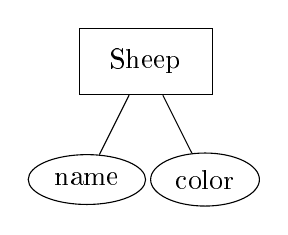
\begin{tikzpicture}
\node[entity] (sheep) {Sheep}
child {node[attribute] {name}}
child {node[attribute] {color}};
\end{tikzpicture}

\end{frame}



% All of the following is optional and typically not needed. 
\appendix
\section<presentation>*{\appendixname}
\subsection<presentation>*{For Further Reading}

\begin{frame}[allowframebreaks]
  \frametitle<presentation>{For Further Reading}
    
  \begin{thebibliography}{10}
    
  \beamertemplatebookbibitems
  % Start with overview books.

  \bibitem{Author1990}
    A.~Author.
    \newblock {\em Handbook of Everything}.
    \newblock Some Press, 1990.
 
    
  \beamertemplatearticlebibitems
  % Followed by interesting articles. Keep the list short. 

  \bibitem{Someone2000}
    S.~Someone.
    \newblock On this and that.
    \newblock {\em Journal of This and That}, 2(1):50--100,
    2000.
  \end{thebibliography}
\end{frame}

\end{document}
